En este capítulo se describirá el análisis económico que se ha llevado a cabo para determinar la viabilidad del desarrollo de este proyecto de manera profesional.

\section{Fuentes de ingreso}
Las posibles fuentes de ingreso que se han barajado se describen en la siguiente lista:
\begin{itemize}
\item \textbf{Vender la propia app}: La solución más obvia, pero quizás no la mejor, es simplemente vender la aplicación en las tiendas digitales para móviles como Google Play Store o su equivalente en iOS, Apple Store. La barrera de tener que pagar para probar la aplicación podría reducir considerablemente el número de usuarios que participarían en la aplicación.

\item \textbf{Google ads}: Una manera de generar ingresos podría ser incluir Google Ads a la aplicación. De esta manera no perderíamos cuota de usuarios y generaríamos unos ingresos proporcionales a la cantidad de usuarios que la utilicen. Además, esta opción cuenta con otra ventaja, y es la de poder dirigir los anuncios en función de la localización del usuario. Pudiendo publicitar lugares que se encuentren físicamente cerca del usuario potenciando los efectos de esta.

\item \textbf{Publicidad de empresas locales}: Esta manera de generar ingresos consistiría en contactar con lugares de ocio de la Isla, como pueden ser centros comerciales, parques de atracciones, zoológicos, actividades, etc. O incluso, de gastronomía, como restaurantes de comida típica canaria. Y colocarlos como punto de interés dentro del mapa de la aplicación, por lo que los usuarios verían ese punto en el catálogo de lugares y, si quisieran completar el mapa de la Isla deberían, al menos, acercarse al lugar. Esto podría ser un incentivo más para que los usuarios visiten esos lugares de ocio y posiblemente generar ingresos en esos lugares o al menos, aumentar el número de personas que transitan por esa zona. Se podrían establecer contratos temporales con las marcas, y que, al finalizar el contrato, ese punto de interés desapareciera del mapa del juego.

\item \textbf{Subvención del Gobierno o del Cabildo}: Quizás sería posible contactar con el Gobierno o el Cabildo de Canarias para ofrecerles participar en el proyecto para fomentar el turismo en la Isla. También se podría exportar fácilmente la app a otras Islas o simplificarla haciendo, por ejemplo, que sea un mapa turístico detallado, de ciudades importantes como Santa Cruz de Tenerife o La Laguna, incluyendo plazas, monumentos históricos, esculturas, etc.
\end{itemize}

Cabe destacar, que se podría hacer una combinación de estas soluciones, es decir, podríamos tener la app con publicidad de Google Ads y con lugares promocionados y ofrecer a los usuarios una versión "premium" sin publicidad.

\section{Desarrollo del proyecto}

En esta sección responderemos a las preguntas: ¿Cuánto cuesta desarrollar este proyecto? ¿Cuánto tiempo tardaría en llevarse a cabo de forma profesional el proyecto? ¿Cuándo se recuperaría la inversión inicial?

Para responder estas preguntas he utilizado el software ProjectLibre\footnote{\textbf{ProjectLibre}: es un software de administración de proyectos de código abierto programado en Java.}, done he creado un proyecto, y añadiendo, los costes estimados y la duración estimada de cada tarea se ha calculado la duración estimada del proyecto, el costo estimado y el camino crítico\footnote{\textbf{Camino crítico}: es la sucesión de tareas que marcan el inicio y el fin del proyecto, por lo tanto, son las tareas que siempre que se retrasen producirán un retraso en la fecha de finalización del proyecto.} de este\footnote{Si desea leer con mayor detenimiento la estructuración de las tareas que componen el proyecto, el archivo que las contiene está disponible en el \href{https://github.com/AaronJoseCabreraMartin/TFG-DiscoverTenerife}{GitHub del proyecto}}.

El proyecto ha sido planteado para estar dividido en cuatro etapas:
\begin{itemize}
\item \textbf{Análisis}: En esta primera etapa se llevará a cabo un estudio de mercado en el que se incluirán tareas como: desarrollo de un análisis PEST, un análisis DAFO, un estudio sobre la identificación de la competencia y un estudio de perfiles de usuarios. También se realizará un diagrama de casos de uso UML y, para finalizar esta etapa, la creación de un documento de análisis de requerimientos. Esta etapa durará un total de 45 días.

\item \textbf{Diseño}: En esta segunda etapa se realizará el diseño completo de la base de datos, la elección del hardware y software a utilizar durante el proyecto y, por último, el diseño de las reglas del juego; cuánta puntuación se obtiene por visitar un lugar, cuánta puntuación se obtiene  por completar un reto, etc. Esta etapa durará un total de 8 días.

\item \textbf{Desarrollo}: Esta segunda etapa es la más se alarga en el tiempo de todo el proyecto. En esta etapa se implementará el diseño de la base de datos realizado en el apartado anterior, se realizará todo el proceso de extracción de información de la web: creando el web scraper, realizando una limpieza de los datos obtenidos y subiendo la información correctamente estructurada a la base de datos. También se realizará el diseño de la interfaz gráfica tanto de la página web como de la aplicación móvil. Y, la última parte, la más importante y larga en el tiempo, la creación de la página web y de la aplicación. Esta etapa dura un total de 65 días.

\item \textbf{Despliegue}: En esta última etapa se incluye la fase de pruebas intensivas a los cuatro sectores del proyecto, al servidor, a la página web, a la aplicación de Android y a la aplicación de iOS. Además, también se incluye la subida de la aplicación a las plataformas de descarga de aplicaciones anteriormente mencionadas, Google Play Store  y Apple Store, con el consecuente cambio a modo de producción. En este punto el proyecto comienza a generar dinero, pero, también en este punto, se añaden los gastos de producción, como son el mantenimiento de Firebase y el mantenimiento de la aplicación, con actualizaciones que corrijan posibles errores, etcétera.
\end{itemize}

\begin{figure}[H]
    \centering
    \includegraphics[width=1\textwidth]{Memoria_TFG_LaTeX/images/Gantt1AnalisisDiseño.png}
    \caption{Primera parte del diagrama de Gantt. En este se muestran las fases de análisis y diseño}
    \label{fig:ganttAnalisisDiseño}
\end{figure}

\begin{figure}[H]
    \centering
    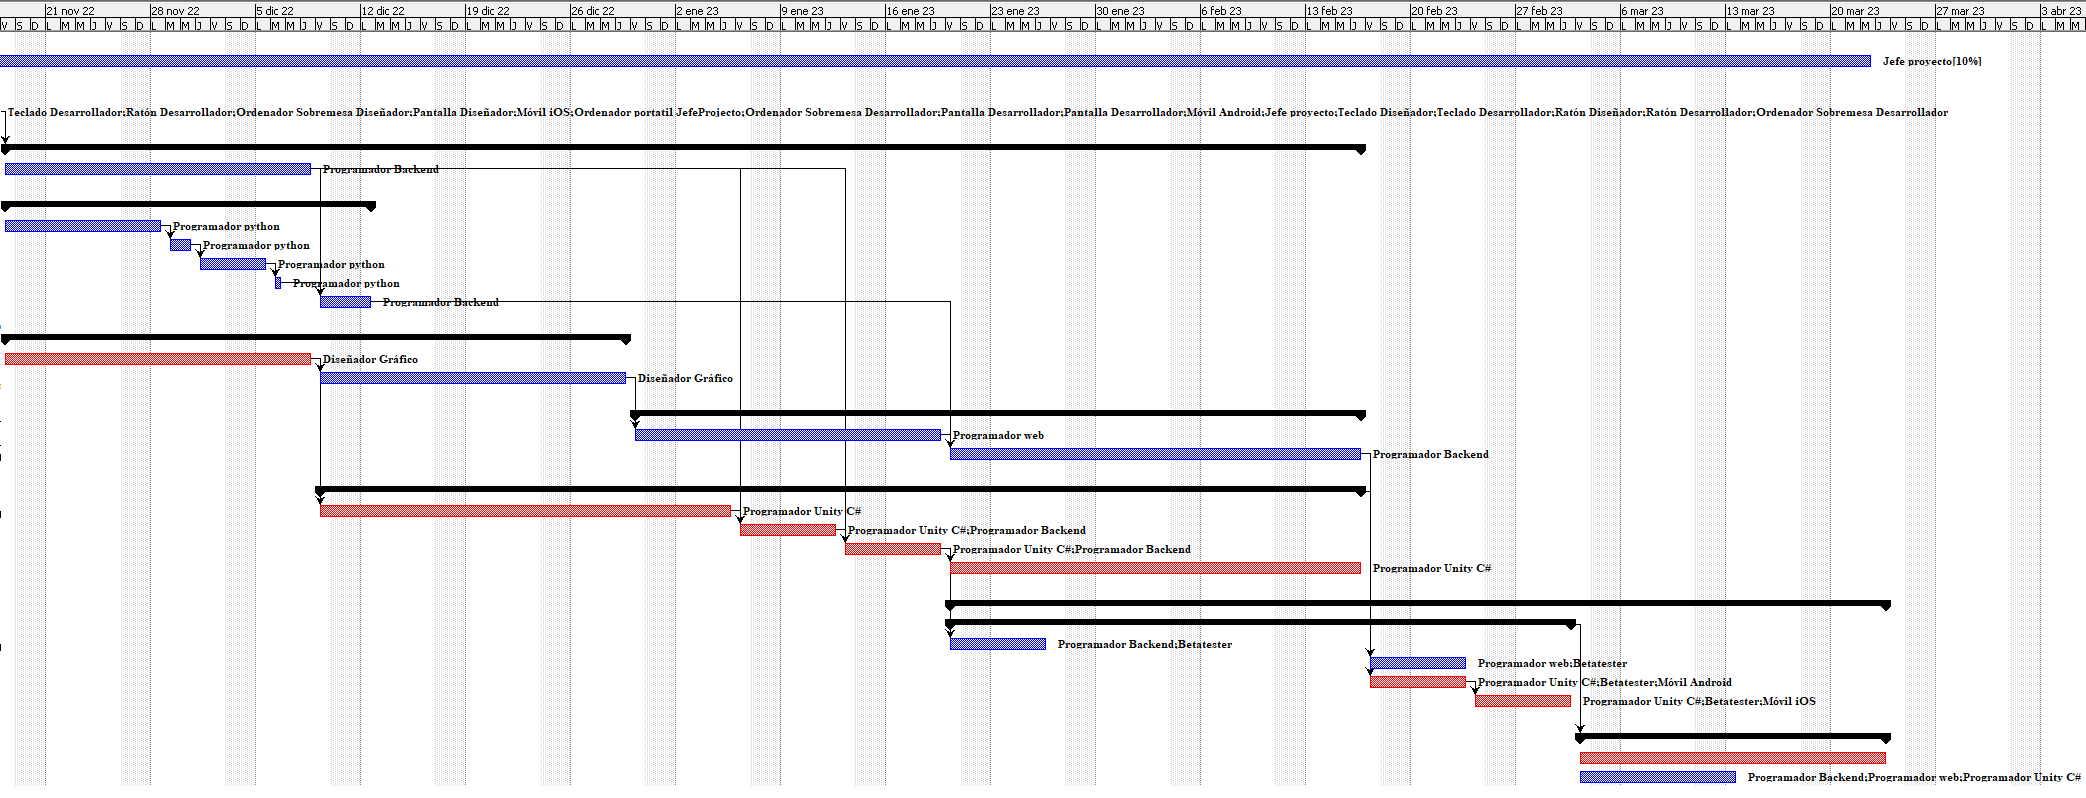
\includegraphics[width=1\textwidth]{Memoria_TFG_LaTeX/images/Gantt2DesarrolloDespliegue.png}
    \caption{Segunda parte del diagrama de Gantt. En este se muestra las fases de desarrollo y despliegue.}
    \label{fig:ganttDesarrolloDespliegue}
\end{figure}

Si se desea observar mejor el diagrama de Gantt o la tabla de recursos, estos están disponibles tanto en forma de imagen como en proyecto de ProjectLibre en el repositorio del proyecto.

\section{Costo y duración del proyecto}

\begin{figure}[H]
    \centering
    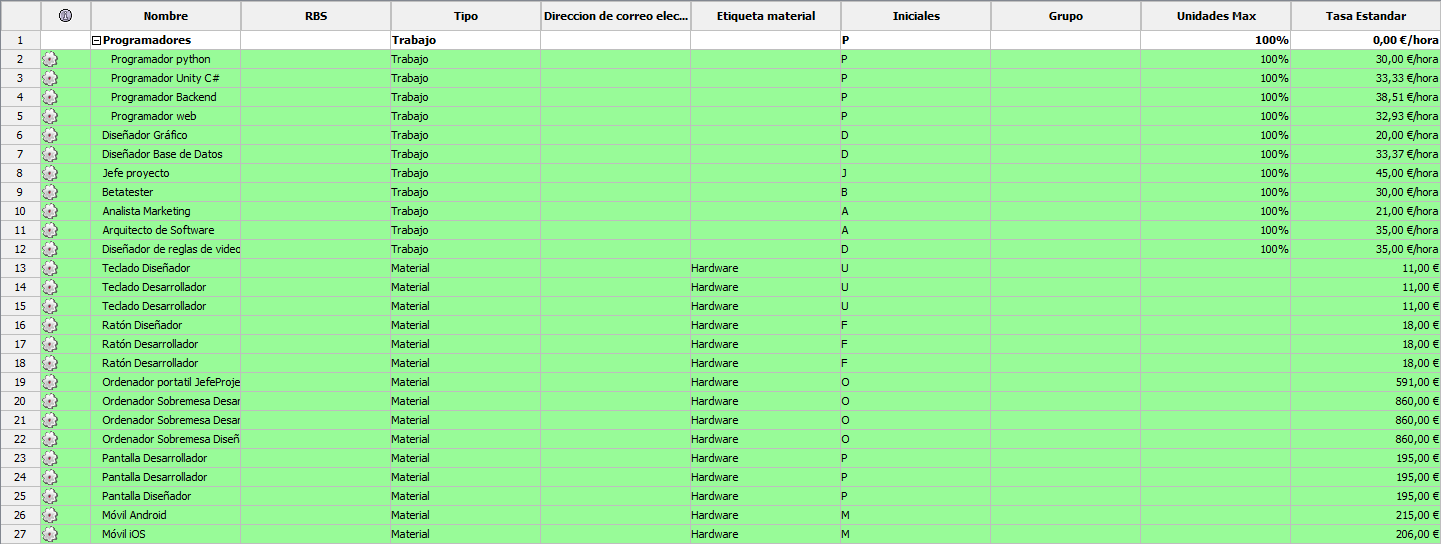
\includegraphics[width=1\textwidth]{Memoria_TFG_LaTeX/images/Recursos.png}
    \caption{Tabla de Recursos tanto materiales como recursos humanos utilizados durante el desarollo del proyecto con sus respectivos costes de uso.}
    \label{fig:tablaRecursos}
\end{figure}

Tras realizar los cálculos de la aproximación de la duración estimada del proyecto, he calculado que el proyecto tardaría 7 meses en terminar su etapa final de creación, el despliegue, y tendría una inversión inicial estimada de, 80569,16 €.

\section{Punto estimado del retorno de la inversión inicial y producción}

En esta fase del proyecto, la aplicación ya está en el mercado y se deben añadir los ingresos que se van generando y los costos de mantenimiento de esta, los cuales, no han sido contabilizados en la inversión inicial.

Para llevar a cabo esta aproximación de los ingresos generados y de los costos de mantenimiento, se ha tenido que aproximar la cantidad de usuarios activos semanales de las dos versiones de la aplicación móvil, Android e iOS, y de la página web.



Con el estudio realizado\footnote{Si desea comprobar el estudio realizado se puede comprobar en el siguiente \href{https://docs.google.com/spreadsheets/d/1Xp9dhk1jerlhGhqqkd2Uu2R6KGxOjXPJQnaUy1ktfSA/edit?usp=sharing}{enlace}.}, se ha demostrado que el proyecto alcanzaría su punto ROI\footnote{\textbf{ROI}: Retorno de Inversión, o por sus siglas en inglés Return Of Investment. Es el instante de tiempo en el cual, el dinero invertido en el proyecto se iguala con el dinero generado por el proyecto.} en la semana número 86 desde el paso a producción, es decir, se tardarían unos 22 meses en recuperar la inversión inicial. A partir de ese punto, el proyecto generaría beneficios para sus inversores. 

\begin{figure}[H]
    \centering
    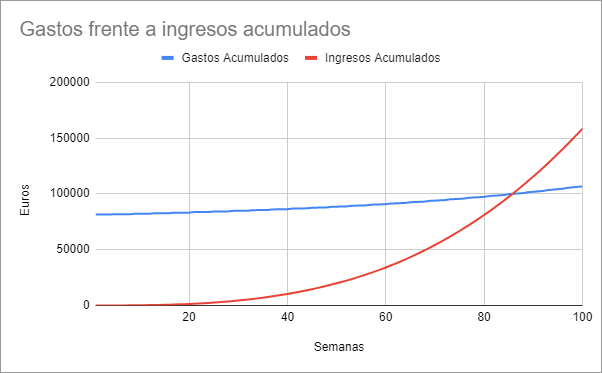
\includegraphics[width=1\textwidth]{Memoria_TFG_LaTeX/images/puntoROI.png}
    \caption{Gráfico en el que se muestra el momento en el cual se alcanza el punto ROI}
    \label{fig:puntoROI}
\end{figure}

Cabe señalar que no se han considerado colaboraciones con empresas locales, establecimientos de interés turístico ni subvenciones del gobierno. Estos ingresos añadidos podrían adelantar en el tiempo el punto ROI.